\subsection{Firestorage}

A desenvolvedora do \textit{Flutter} e do \textit{Firebase} é a mesma, neste sentido, disponibilizou recursos que facilitam a utilização desta ferramenta pelo \textit{Flutter}. Sendo assim, todas as imagens e vídeos de utilizadores, tópicos e comentários são guardados diretamente da aplicação para o \textit{Firestorage}, assim como, o acesso às mesmas é realizado diretamente.

Para permitir este tipo de acesso o \textit{Firebase} disponibiliza uma ferramenta que possibilita, que através do terminal se realize a configuração da ligação entre o projeto e o servidor do \textit{Firebase}, sendo que, no final apenas é necessário importar a biblioteca do serviço do \textit{Firebase} que se deseja e invocar a classe do mesmo para serem realizadas ações.

Os ficheiros são organizados conforme o seu contexto. Para utilizadores, existe a pasta utilizadores, para tópicos, existe a pasto tópicos e para comentários, existe a pasta comentários. 


A pasta utilizadores, como cada utilizador, apenas contém uma imagem, então são guardadas com o nome do \textit{id} do utilizador e na eventualidade de já existir é substituída. No caso de tópicos e comentários, como podem conter várias imagens e vídeos, estes são guardados em pastas com os ficheiros referentes, que têm como nome os \emph{id's} dos tópicos ou comentários.

\begin{figure}[htb]%
 \centering
 \subfloat[\centering Raiz do Firestorage]{{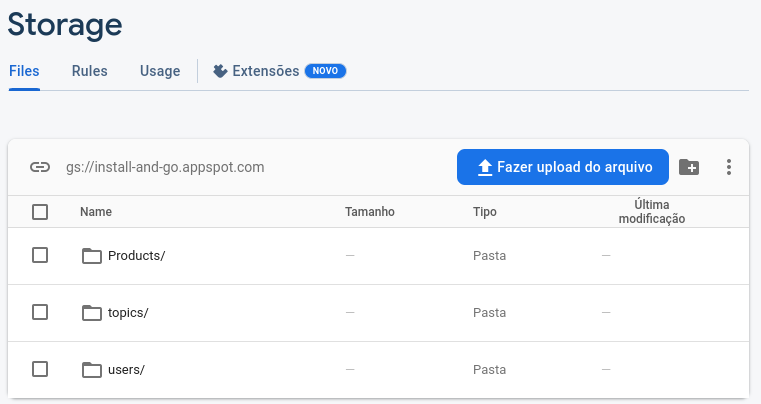
\includegraphics[width=0.7\textwidth]{images/implementacao/frontend/firestorage/all.png} }}%
 \qquad
 \subfloat[\centering Pasta topics do Firestorage]{{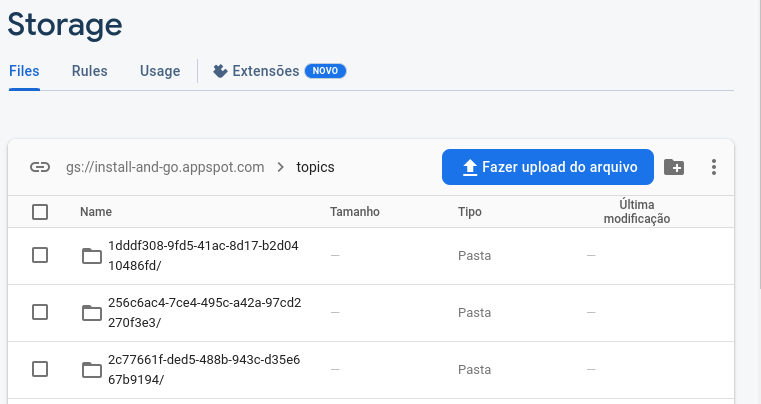
\includegraphics[width=0.7\textwidth]{images/implementacao/frontend/firestorage/topics.png} }}%
 \label{fig:76}%
\end{figure}